\documentclass[sigconf,anonymous,review,balance=false]{acmart}
\usepackage{popets}
\usepackage{amsmath}
\usepackage{array}

% Copyright
\setcopyright{popets}
\copyrightyear{2027}

% Issue info
\acmYear{2027}
\acmVolume{2027}
\acmNumber{3}
\acmDOI{XXXXXXX.XXXXXXX}
\acmISBN{}
\acmConference{Proceedings on Privacy Enhancing Technologies}
\settopmatter{printacmref=false,printccs=false,printfolios=true}

\definecolor{leakred}{HTML}{B23A48}
\newcommand{\canary}{\texttt{CANARY-BC267061-\allowbreak 67DC-485B-8E51-6F5494765CAB}}

\begin{document}

\title[Warning: Do Not Upload This to an LLM Tool!]{Warning: Do Not Upload This to an LLM Tool!}
\subtitle{Measuring Data Exposure in LLM-Integrated Productivity Tools}

\author{Marawan Eldeib}
\orcid{0009-0008-5285-424X}
\affiliation{%
  \institution{Master INFOTECH, University of Stuttgart}
  \city{Stuttgart}
  \country{Germany}}
\email{marawandeep13@gmail.com}

\author{Marco Aiello}
\orcid{0000-0002-0764-2124}
\affiliation{%
  \institution{University of Stuttgart}
  \city{Stuttgart}
  \country{Germany}}
\email{marco.aiello@iaas.uni-stuttgart.de}

\renewcommand{\shortauthors}{Eldeib and Aiello}

\begin{abstract}
Confidential material increasingly arrives with an instruction not to feed it to any
LLM-based service: reviewers of papers and grant proposals, for instance, are now commonly
bound by such terms. We ask whether a user who follows that instruction can be confident
that the document has not been shared. LLM-integrated productivity tools, browser
extensions, desktop assistants, and cloud-connected office suites, observe content without
being invoked, so a document may be transmitted to several third-party providers simply
because it was opened or pasted into an ordinary text field. We quantify this exposure with
an HTTPS interception proxy and a synthetic confidential memo carrying twelve unique planted
identifiers, including a UUID canary, so that every transmitted fragment is attributable to
our input. In a controlled browser experiment, two writing-assistant extensions, Grammarly
and LanguageTool, transmitted essentially the entire document (99.0\% and 91.9\% of
characters) and all twelve identifiers on every run, while a no-extension baseline
transmitted nothing. Extending the measurement to desktop and office surfaces shows that
exposure is surface-dependent rather than storage-dependent: a PDF merely opened in a
viewer without an assistant transmitted nothing, whereas opening the same content as a
\texttt{.docx} in Microsoft Word with connected experiences enabled streamed 96.8\% of it
to a Microsoft endpoint with no further user action; Word's Protected View contained Microsoft's own channel but not a
third-party desktop assistant; and a Copilot reply that declined to reveal the secrets came
after they had already been sent. A single Office setting removed the largest incidental
transfer. We frame the results as a gap between documented default behaviour and reasonable
user expectation rather than as a vulnerability. All test data is synthetic and the
measurement pipeline is released.
\end{abstract}

\keywords{Browser extensions, data exposure, HTTPS interception, LLM-integrated productivity tools, PII leakage}

\maketitle


\section{Introduction}
\label{sec:intro}

Much of the material that reaches us in professional life arrives with a restriction on
what we may do with it. A manuscript under review for a conference or journal, a grant
proposal sent to an external evaluator, a draft contract, a patient record, a student's
thesis: each is confidential by default and, increasingly, carries an explicit instruction
that it must not be uploaded to a large-language-model (LLM) based service. Publishers and
funding agencies now write such prohibitions into their reviewer guidelines; the National
Institutes of Health, for example, bar the use of generative AI tools in any part of their
peer-review process on confidentiality grounds~\cite{nih2023genai}. Reviewers routinely
accept these terms and most would say that they honour them: they do not paste the paper
into a chatbot.

The question this paper asks is whether that confidence is warranted. The modern desktop
is saturated with LLM-integrated services that observe content without being invoked, and
they are not confined to any one product category. Machine-translation clients upload the
text they are given in full. AI ``helpers'' embedded in applications, the assistant in the
office suite, the copilot in the browser, the summariser in the PDF viewer, read the open
document to offer their suggestions. Cloud-connected office suites stream opened files to
analysis endpoints as a default ``connected experience.'' Writing assistants attach
themselves to every editable field in the browser or to whatever window has focus. None of
these requires the user to decide to share anything. A reviewer who opens the proposal as a
Word attachment, or who types a few sentences of assessment into the review form while a
writing assistant is enabled, may have transmitted the document, in whole or in substantial
part, to third-party providers none of which they consciously chose. The prohibition on
uploading the paper to an LLM assumes a deliberate act; the exposure we study happens
without one. Where exactly the line falls, which actions on which surfaces transmit and
which do not, is what this paper sets out to measure.

This concern is not hypothetical. \citet{vekaria2025bighelp} audited nine generative-AI
browser assistants and showed, by decrypting their traffic, that several forward full page
content, including medical and financial details, to their own servers and to third-party
trackers, and use it for profiling. That work established that the problem exists across a
class of tools. Here we take the next step and ask, for a single confidential document and
under controlled conditions, exactly how much of it leaves the machine, through which
surface, triggered by which user action, and whether the user can switch the channel off.
As the primary use case we take grammar checkers, and Grammarly in particular: they are
among the most widely installed LLM-integrated tools, they run permanently in the
background rather than on demand, and they are precisely the kind of software a
conscientious reviewer would not think of as ``an LLM tool.'' We then extend the
measurement to a translator, an office suite, a browser copilot, and a desktop assistant,
so that the result is about the class of tools rather than one product. Concretely, this
paper makes the following contributions.

\begin{itemize}
  \item \textbf{A canary-based, per-secret measurement method.} We plant twelve unique
        synthetic identifiers, including a UUID canary, in a confidential memo and score
        every decrypted client-to-server flow for character coverage and for each secret
        individually, against a no-extension baseline and with proxy-free corroboration.
        Every transmitted fragment is thereby unambiguously attributable to our input,
        which large-scale crawls cannot offer.
  \item \textbf{A controlled comparison of two writing-assistant extensions.} Under
        identical paste conditions, Grammarly and LanguageTool transmitted essentially the
        entire document (99.0\% and 91.9\% of characters) and all twelve secrets on every run,
        while the baseline transmitted nothing.
  \item \textbf{An exposure taxonomy across surfaces beyond the browser.} We distinguish
        user-initiated, incidental, and passive exposure and measure each across a
        translation client, Microsoft Office, Edge/Copilot, and a desktop assistant.
        Exposure turns out to be surface-dependent, not storage-dependent: a file on a USB
        stick or in a synced cloud folder transmits nothing until its content enters a
        surface an LLM-integrated service watches. Among the surface-specific findings, a
        PDF opened in a plain viewer transmitted nothing, whereas opening a \texttt{.docx}
        in Word with connected experiences enabled streamed 96.8\% of the document to a
        Microsoft endpoint with no further user action; Word's Protected View
        contained Microsoft's own channel but not a third-party desktop assistant, which
        still transmitted 94.2\%; and Copilot's visible refusal to reveal the planted secrets
        came after all twelve had already been sent.
  \item \textbf{Mitigation and channel analysis.} A single Office privacy setting removed the
        largest incidental transfer, and a permission audit shows the exposure channel is the
        tools' all-sites text access rather than any sensor capability.
\end{itemize}

The tools we study behave as their vendors document. Our contribution is not a
vulnerability but a quantified account of the distance between that documented behaviour
and the expectation of a user who has been told, and believes, that the document has not
been shared. All test data is synthetic, and the capture and scoring pipeline is released
for reproduction.

The remainder of the paper is organised as follows. Section~\ref{sec:related} reviews how
LLM-integrated tools obtain and transmit content and surveys the state of the art in
extension and assistant privacy measurement. Section~\ref{sec:threat} defines the three
modes of exposure and the threat model. Section~\ref{sec:method} describes the test
document, the interception setup, and the metrics. Section~\ref{sec:results} reports the
controlled browser experiment and the host-level measurements, and
Section~\ref{sec:discussion} discusses their implications, including the regulatory
context. Section~\ref{sec:limitations} states the limitations, and
Section~\ref{sec:conclusion} concludes.

\section{State of the Art}
\label{sec:related}

%\subsection{How LLM-integrated tools obtain content}
%\label{sec:background}
LLM-integrated productivity tools reach user content through three integration types. A
browser extension registers content scripts that attach to a page's editable
fields (\texttt{<textarea>} and \texttt{contenteditable} elements) on visited pages. When
text appears in such a field, the extension transmits it, typically over HTTPS or a
WebSocket, to its backend, which runs the analysis and returns suggestions. A desktop
assistant or translation client reads the text of the focused window or of the clipboard
and sends it to a cloud service. An office suite or a browser with a built-in copilot reads
the opened document itself, either as a background ``connected experience'' or when the
user invokes the assistant. Because the analysis is server-side, the text must leave the user's machine for
the feature to function at all.

\subsection{State of the art}

\paragraph{Privacy leakage by browser extensions.}
The privacy risks of browser extensions have been studied for the better part of a decade.
\citet{starov2017extended} were among the first to systematically measure the ``privacy
diffusion'' enabled by extensions, showing that many leak identifying information far
beyond what their function requires. \citet{weissbacher2017exray} built Ex-Ray to detect
history-leaking extensions, \citet{aggarwal2018ispy} detected extensions that covertly
exfiltrate browsing behaviour, and \citet{chen2018mystique} scaled dynamic taint tracking
to 181{,}683 extensions, flagging thousands that leak privacy-sensitive information. Static
data-flow analysis (DoubleX~\cite{fass2021doublex}) later added scale on the code side.
These works established that extension data collection is widespread and frequently
undisclosed, and introduced the complementary detection methods the field still relies on:
differential string search, content-agnostic network analysis, and taint tracking. They
rest on a longer study of the extension security model itself:
\citet{carlini2012chrome} showed that over-broad host permissions undercut Chrome's
isolation guarantees, and \citet{pantelaios2020changed} showed that benign extensions can
turn malicious through later updates, which is why a runtime, network-level measurement of
what a tool actually transmits is more reliable than trusting a reviewed snapshot.

More recent large-scale studies have moved from browsing metadata to page content.
\citet{nayak2024experimental} analysed sensitive-data access by extensions across the
Chrome Web Store, including access to credentials on login pages. \citet{xie2024arcanum}
built Arcanum, a dynamic taint-tracking system, and found that thousands of extensions, used
by an estimated 144 million people, collect on-page content such as email bodies and
banking information, often without accurate disclosure. Closest to our design,
\citet{bui2023extpriva} intercepted the network traffic of roughly 47{,}000 extensions and
compared the observed outbound flows against each extension's stated privacy practices,
finding hundreds whose transmissions contradicted their disclosures. From the tracking
side, \citet{dambra2022sally} measured web tracking from the user's perspective, building on
the browser-instrumentation paradigm established by OpenWPM~\cite{englehardt2016openwpm}.

\paragraph{Exfiltration before the user acts.}
The most behaviourally similar precedent is ``read-before-submit'' exfiltration.
\citet{senol2022leakyforms} showed that email addresses and even passwords are sent to
third parties as the user types, before any form is submitted; \citet{munir2025keystroke}
generalised this, finding widespread third-party keystroke event-listener interception
across popular sites; and \citet{starov2016contactforms} earlier quantified PII leaking
from website contact forms. We extend the ``transmitted before the user acts'' framing from
trackers embedded in pages to assistants installed by the user.

\paragraph{Network-level PII measurement.}
Methodologically, our detection step, searching intercepted flows for known sensitive
strings, follows a mature lineage rooted in dynamic taint tracking
(TaintDroid~\cite{enck2010taintdroid}) and network-level flow analysis over decrypted
mobile traffic (ReCon~\cite{ren2016recon}). Because outbound payloads can be encoded or
obfuscated, we adopt unique planted canaries in the spirit of the black-box differential
leak detection introduced by AGRIGENTO~\cite{continella2017agrigento}, so that any
transmitted fragment is unambiguously attributable to our input. Interception itself can
weaken the observed connection~\cite{durumeric2017https}, a limitation we return to in
Section~\ref{sec:limitations}.

\paragraph{Generative-AI assistants.}
The work closest to ours is that of \citet{vekaria2025bighelp}, who audited nine
generative-AI browser assistants and, using traffic decryption, showed that several forward
full webpage content, including medical and banking details, to their own servers and to
third-party trackers, and that some profile users across sessions. Our study is narrower
and complementary. Where that audit characterises what a class of assistants collects across
browsing, we measure, for one confidential document, how much of it leaves and through which
channel, with each transmitted fragment attributable to our input through planted canaries;
we separate the user action that triggers each transfer; and we extend the measurement from
the browser to desktop clients and the office suite, which a browser-only audit cannot
reach. A 2026 consumer-privacy ranking of AI-powered Chrome extensions places Grammarly and
QuillBot among the highest-risk by declared data collection~\cite{incogni2026ranking},
which motivates our choice of grammar checkers as the primary case. Industry reporting corroborates the class of behaviour: a Unit~42 investigation found
``productivity'' extensions that read users' email as they write it~\cite{unit42genai2026},
and enterprise-security analyses note that such extensions read page content largely
invisibly to standard data-loss-prevention tooling, much of it from personal, unmonitored
accounts~\cite{csa2026extensions,cyberhaven2026}.

\paragraph{What happens after transmission.}
Why the transmitted content matters is reinforced by work on the privacy risks of the
language models that sit behind these assistants. \citet{carlini2021extracting} showed
that language models memorise and can regurgitate verbatim personal data from their
training set, and \citet{nasr2025scalable} extended such extraction to aligned production
models; \citet{lukas2023pii} quantified PII leakage from language models and showed that
scrubbing and differential privacy leave residual exposure. \citet{staab2024beyond} showed
that models infer sensitive attributes from ordinary prose, and
\citet{mireshghallah2024cansecret} that LLM-integrated applications routinely disclose
information to recipients inappropriate for the context. Threat-intelligence reporting has
found deployed AI services and unauthorised ``model-reseller'' proxies silently storing and
passing on users' inputs~\cite{anthropic2026threats}. Text sent to a writing assistant is
therefore not inert once it leaves the machine. The gap between what users believe about
their exposure and what actually leaves their devices has itself become a subject of study:
recent work frames a ``privacy paradox'' between user perceptions and the reality of PII
leakage in LLM-integrated settings~\cite{privacyparadox2026}. Our framing of that gap
follows Nissenbaum's contextual integrity~\cite{nissenbaum2004contextual}: the flows we
measure carry information into a context the user did not intend.

\paragraph{Research gap.}
Prior work either counts how many extensions leak at scale, or audits AI assistants that
the user invokes. What is missing is a controlled, canary-proven, per-secret measurement of
how much of a single confidential document leaves the machine, across both the browser
extensions and the everyday host applications a user encounters, with the user action that
triggers each transfer identified. This paper fills that gap.

\section{Threat Model}
\label{sec:threat}

%\subsection{Modes of exposure}
\label{sec:modes}
A user's text can reach one of these tools in three ways, and this study measures all
three. In \emph{user-initiated} exposure, the user knowingly hands the text over: they
paste into the tool's own editor or click an action such as ``translate'' or
``summarise.'' Transmission is expected, but its extent is not; how much of a document a
tool ships once invoked is itself a privacy-relevant quantity. In \emph{incidental}
exposure, the tool is installed and enabled, and it captures text the user entered or
opened for an unrelated purpose, with no intent to use the tool and no action beyond typing,
pasting, or opening a file. In \emph{passive} exposure, the document is merely present on
the machine, stored on a removable drive or in a synced folder, and the question is whether
anything reads it. The second mode is our primary scenario, because the disclosure happens
with no step the user would recognise as sharing; the first and third bound it from either
side.

%\subsection{Threat model}
We model an ordinary, non-adversarial situation. A user receives a confidential file and is
explicitly told not to share it with AI tools. They have a writing-assistant extension or
desktop client installed and enabled by default. In the course of normal work they open the
file, or paste part of it into an ordinary text field (an email reply, a review form, a
notes box). Without any further action, the tool transmits the content to its servers.

We do not assume a malicious vendor, a compromised endpoint, or a network attacker. The
concern is unintended disclosure of document content to remote service providers through
enabled productivity-tool integrations. Chatbot websites into which a user deliberately
pastes text are out of scope: that is intended use by definition and carries no gap between
behaviour and expectation. The more confidential the work, the more each of the three modes
of Section~\ref{sec:modes} matters.


\section{Methodology}
\label{sec:method}

\begin{figure*}
\centering
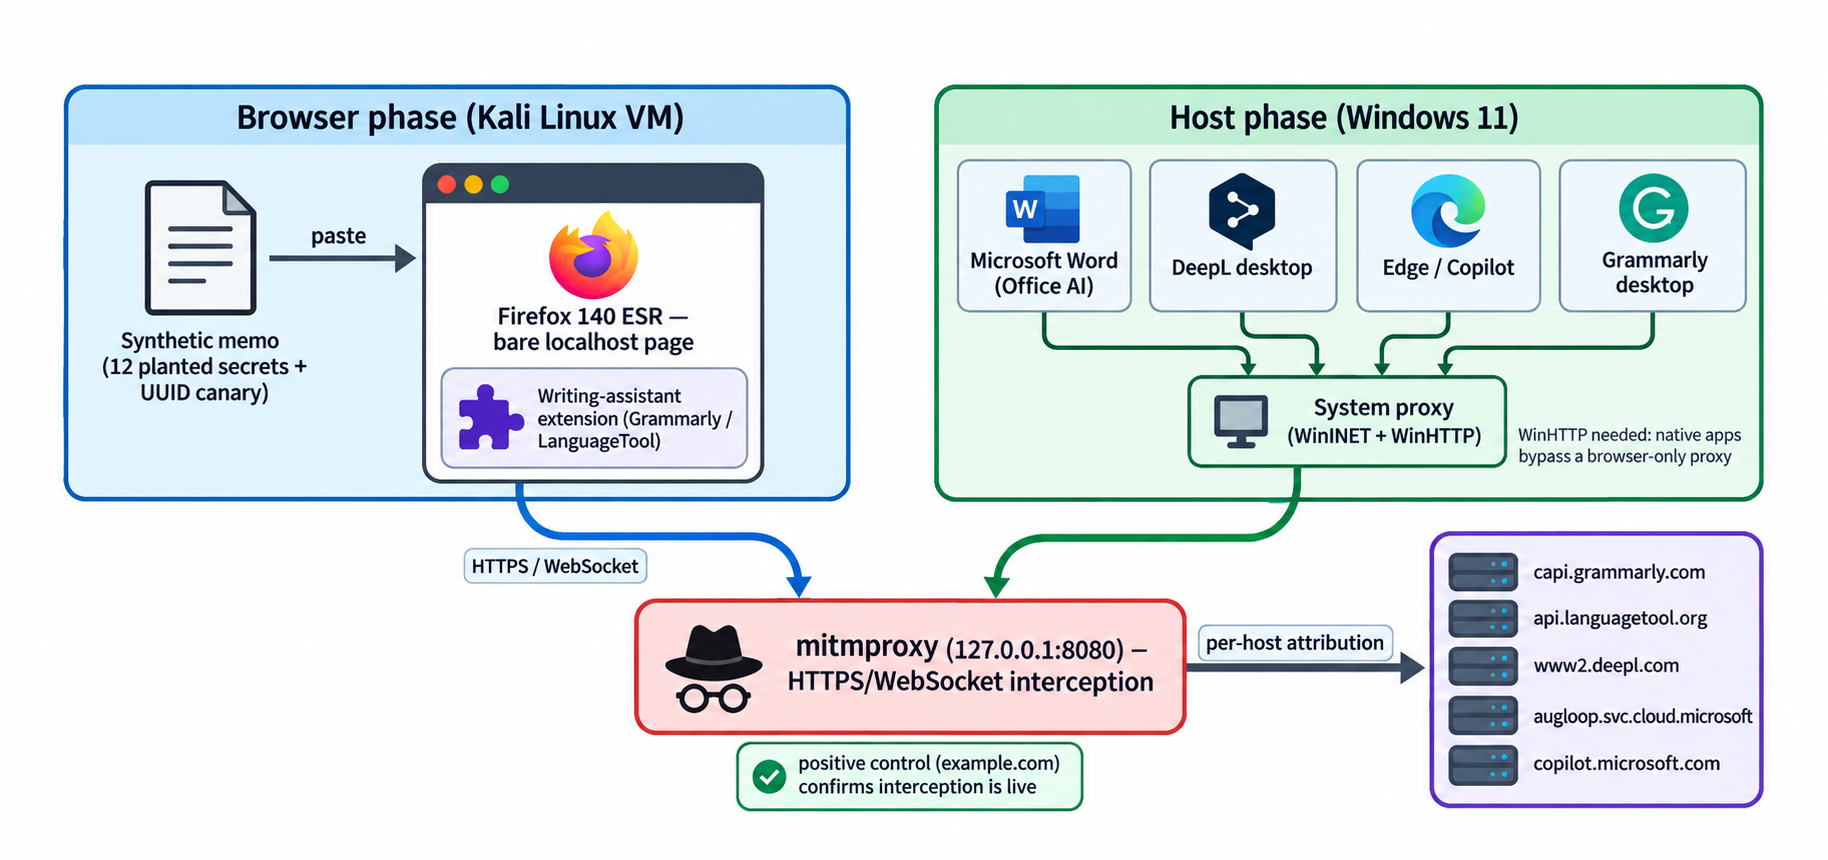
\includegraphics[width=0.92\textwidth]{figures/fig_setup.png}
\caption{Experimental setup. In the browser phase (isolated Kali Linux VM), the synthetic
memo is pasted into a bare local page and read by the writing-assistant extension. In the
host phase (Windows~11), native applications and Office reach the network through the system
proxy (WinINET + WinHTTP, the latter required because native clients bypass a browser-only
proxy). Both phases route through mitmproxy (\texttt{127.0.0.1:8080}); a positive control
(example.com) confirms interception is live, and every flow is attributed to its
destination host.}
\Description{Block diagram: a synthetic memo enters either a browser VM running a writing-assistant extension or a Windows host running Office and desktop clients; both route through a local mitmproxy instance that decrypts and scores outbound flows per destination host.}
\label{fig:setup}
\end{figure*}

%\subsection{Study design and conditions}

The study has two phases. The \emph{primary} experiment is a controlled, same-task browser
comparison of three conditions: Grammarly, LanguageTool (an independent product from LanguageTooler GmbH that
requires no account), and a no-extension baseline (the same browser and steps with no
extension installed, a negative control for the browser's background traffic). Two
independent tools guard against attributing to the class what is a quirk of one product. The \emph{secondary},
exploratory host phase then probes several other surfaces: the DeepL desktop client, Microsoft~Word
with Office connected experiences, the Grammarly desktop client under Protected View,
Edge/Copilot on a PDF, and passive conditions (storage only, or viewers without an assistant); these conditions differ in user action and file format, so they are read
individually rather than as a same-task cross-tool comparison. Together the conditions
cover the browser-extension, desktop-application, and editor/Office integration types.
Software versions and accounts for both phases are listed in Table~\ref{tab:env}.

\begin{table}
\centering
\caption{Experimental environment. Host application versions were recorded after the
experiments; because these clients auto-update, earlier host runs may have used slightly
earlier builds.}
\label{tab:env}
\small
\begin{tabular}{@{}ll@{}}
\toprule
\textbf{Component} & \textbf{Version / configuration} \\
\midrule
\multicolumn{2}{@{}l}{\textit{Browser phase (Kali Linux VM)}}\\
Firefox                & 140.12.0esr \\
Grammarly extension    & 8.937.0 (free account, logged in) \\
LanguageTool extension & 11.0.2 (no account) \\
mitmproxy              & 12.2.3 \\
\midrule
\multicolumn{2}{@{}l}{\textit{Host phase (Windows 11 25H2)}}\\
Microsoft 365 (Word)   & 16.0.20326.20144 (Click-to-Run, personal) \\
Microsoft Edge         & 153.0.4234.32 \\
DeepL desktop          & 26.9.1 \\
Grammarly for Windows  & 1.2.296.1955 \\
iCloud Drive           & Advanced Data Protection off \\
\bottomrule
\end{tabular}
\end{table}

\subsection{Test document and planted secrets}

The input is a synthetic ``confidential memo'' (2{,}065 characters, 245 words) written
to look like an internal compliance document and explicitly marked
``\textsc{do not forward}.'' Embedded in its prose are twelve unique,
fictional identifiers: names, an email address, a phone number, project and
reference codes, and a UUID canary, \canary{}. These identifiers are synthetic and were not
intentionally reused from any real source, so any occurrence in captured network traffic is
attributable to our input. The canary in particular is a high-specificity
attribution marker: its appearance in client-to-server traffic is strong evidence that
content from the synthetic document was transmitted toward that service.
Table~\ref{tab:secrets} lists the twelve identifiers and their categories.

\begin{table}
\centering
\caption{The twelve planted identifiers embedded in the synthetic memo.}
\label{tab:secrets}
\small
\begin{tabular}{@{}ll@{}}
\toprule
\textbf{Category} & \textbf{Item} \\
\midrule
Name (direct identifier)      & Helena Voss \\
Name (direct identifier)      & Theodora Baumgartner-Klein \\
Contact detail                & Email address \\
Contact detail                & Phone number \\
Official / ID number          & Employee ID \\
Official / ID number          & Tax registration number \\
Financial identifier          & Q1 expenditure reference \\
Financial identifier          & Reserve fund code \\
Financial identifier          & Budget approval code \\
Legal / contractual reference & Contract number \\
Confidential project ID       & Project codename \\
Canary proof-token            & Unique UUID leak marker \\
\bottomrule
\end{tabular}
\end{table}

\subsection{Interception setup}

For the browser phase, all captures were performed on an isolated Kali Linux virtual
machine so that the man-in-the-middle configuration never touched real browsing. We used
mitmproxy~\citep{mitmproxy} (version 12.2.3) as an intercepting HTTPS/WebSocket proxy
on \texttt{127.0.0.1:8080}. Each tool ran in its own clean Firefox profile with the
proxy configured and the mitmproxy certificate authority trusted only within
that profile, so decryption was scoped to the experiment. Before any data collection,
interception was verified per profile (a known HTTPS site must load without a
certificate warning and appear in the proxy); this guards against the failure mode in
which broken interception is indistinguishable from a genuine zero-exposure result.

The document was pasted into a bare local HTML page containing a single text field and
nothing else (no third-party scripts, analytics, or other domains) served over
\texttt{http://localhost} so that extension content scripts activate exactly as they
would on a real site, but with zero background noise to filter out.

\subsection{Capture procedure}

For each run, the document was loaded into the clipboard and pasted manually into the
focused field, after which the run recorded for sixty seconds. The manual paste matters: a scripted paste fills the field without firing the DOM
\texttt{input} event the extensions listen for, so the tool never ingests the text and
reports a misleading zero. Each tool was captured for
five runs and the baseline for three, following an identical, locked
protocol so that between-run variance measures reproducibility rather than procedural
drift.

\subsection{Host and system-level phase}
Several desktop tools (Microsoft~Office, the DeepL desktop client, Edge/Copilot) are not
available on Linux, so the host phase was run on a Windows~11 laptop using the same
interception principle. mitmproxy ran the same scoring add-on, and both the WinINET and
WinHTTP system proxies were pointed at it, with the mitmproxy CA trusted in the Windows
certificate store and the proxy enabled only during capture. WinINET carries browser and
interactive-app traffic; WinHTTP carries native and background apps. Office and the Grammarly desktop
client use WinHTTP and would bypass a WinINET-only (browser) proxy, so covering both is
what makes the host capture complete. For the storage cases, where the question is whether
a file is actually read rather than what leaves the network, we additionally recorded local
file-access activity with Process Monitor, so we could tell a file being opened from one that was only stored. Each
condition used the same synthetic memo and canary. Because a real machine runs several
assistants at once, every captured flow was attributed to its destination host, so a
transmission is credited to the specific tool responsible rather than to whatever else
happened to be running.

\subsection{Metrics}
\label{sec:metrics}

A mitmproxy add-on scored client-to-server HTTP request bodies and client-to-server
WebSocket frames; server responses were retained in the raw capture for validation but
excluded from exposure scoring, so a backend echoing text back cannot inflate the figure.
The raw captures were also archived so they can be re-analysed offline. We report, in order
of importance:

\begin{description}
  \item[Planted-secret count (primary).] How many of the twelve identifiers reached
        the servers, verified individually. The canary makes this unambiguous.
  \item[Exposure \%.] Character coverage: the fraction of the document's character
        positions covered by at least one matching 20-character window, so that overlapping
        matches contribute each position at most once. Let $\mathcal{T}$ be the set of
        decoded outbound substrings and $w_{20}(i)$ the 20-character window at position $i$;
        the covered set and exposure are
        \begin{align*}
          C &= \!\!\bigcup_{\,i:\,w_{20}(i)\in\mathcal{T}}\!\!\{i,\ldots,i+19\}, \\
          \mathrm{Exposure}\,(\%) &= \frac{|C|}{N}\times 100,
        \end{align*}
        where $N$ is the document length in characters. A 20-character window is long enough
        to avoid false matches from common words and short enough to catch fragmented sends;
        a per-host concatenated-transcript pass (all of a host's traffic joined into one
        stream) additionally catches content split across multiple frames. Matching is
        case-folded and performed over plain, URL-decoded, JSON-unescaped, HTML-entity,
        base64-decoded, UTF-16, and Unicode-NFC variants so that encoded transmission is
        still detected, and compressed bodies (gzip, brotli, zstd) are decoded first.
        Traffic to hosts also seen in the no-extension baseline is discarded only when it
        carries no document coverage and no secret (pure background); a matching flow on a
        host shared with the baseline is never dropped, so baseline subtraction removes
        noise without erasing a genuine transmission.
  \item[Reproducibility and confidence.] We report confidence in two parts:
        \emph{repeatability}, the standard deviation of exposure \% across a condition's
        runs in percentage points (pp), labelled High ($<3$~pp), Medium ($3$--$10$~pp), Low
        ($>10$~pp), or not assessable for single-run conditions; and \emph{capture
        completeness}, complete when no TLS handshake escaped interception and a lower bound
        otherwise.
  \item[Traffic visibility.] Reported as two separate numbers: the share of
        intercepted events that used HTTPS, and the count of TLS handshakes that could not be intercepted, for
        example because of certificate pinning. These
        are never combined into a single
        figure, because a non-zero failure count means the exposure result is a lower
        bound (traffic we cannot decrypt could only add to what was sent, never subtract).
\end{description}

\noindent
Beyond the twelve planted secrets, we also run an automatic PII detector (Microsoft
Presidio~\cite{microsoft2018presidio}) over the decrypted bodies to catch sensitive data we
did not plant; its only finding beyond the planted identifiers, an account token in
Grammarly's traffic, is reported in Section~\ref{sec:linkability}.

\noindent
Where within-setup runs were identical we report the measured exposure directly rather than
as a confidence interval; such run-to-run stability is not a claim of stability across
software versions, accounts, regions, document types, or future server-side behaviour.

\begin{figure*}
\centering
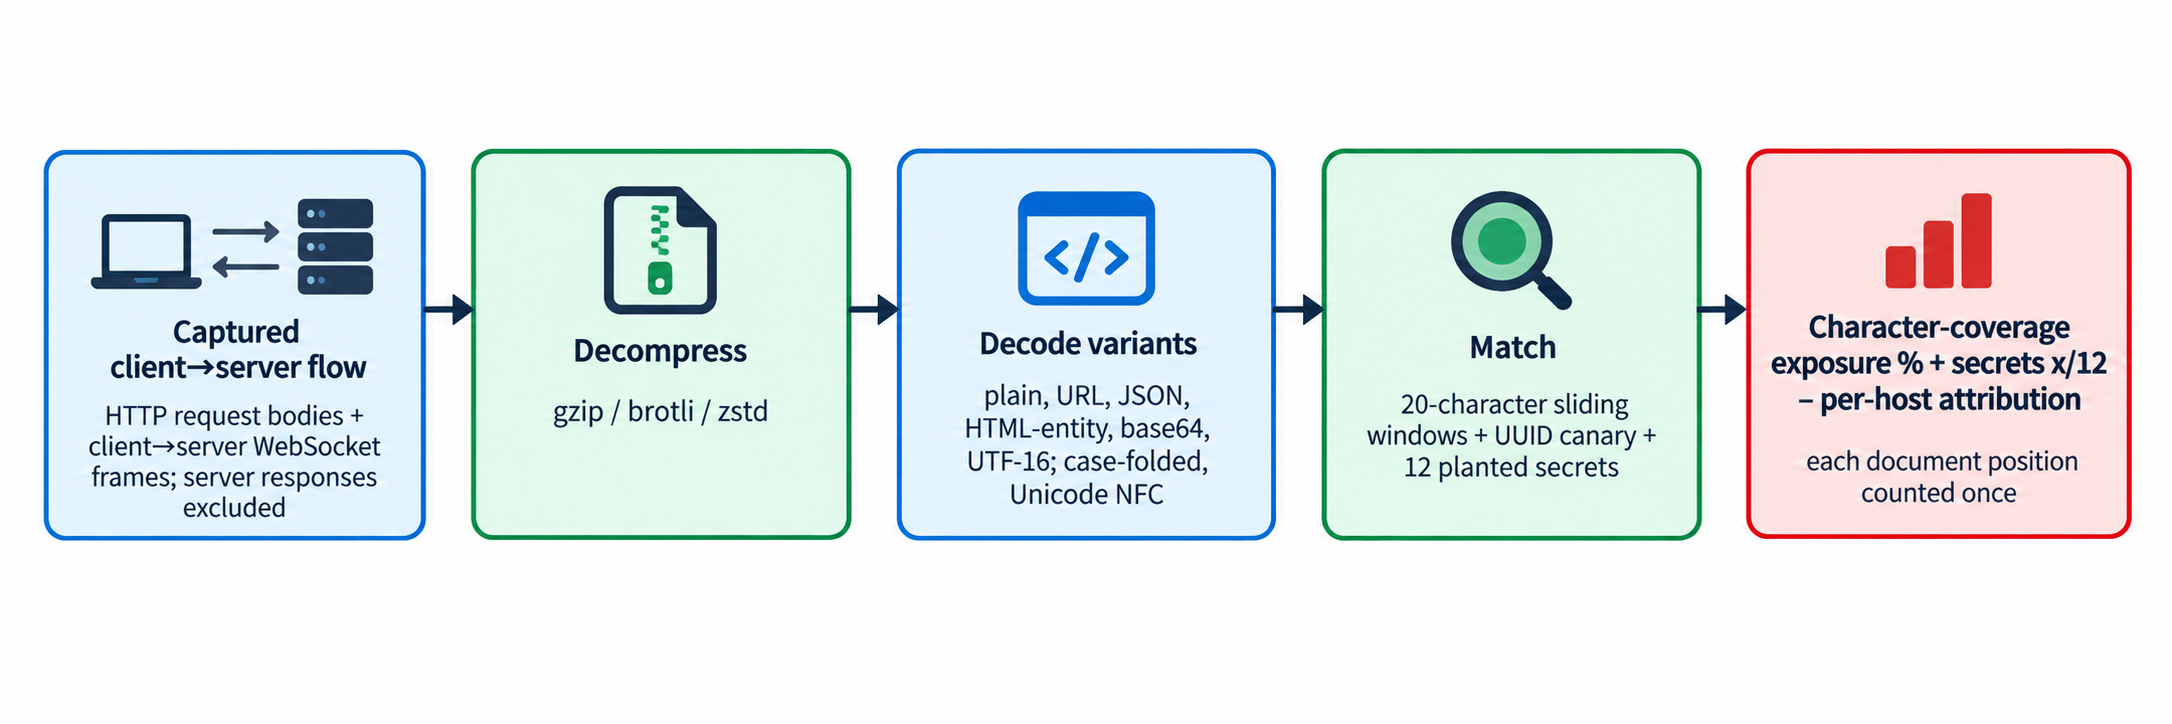
\includegraphics[width=0.92\textwidth]{figures/fig_pipeline.png}
\caption{Exposure-scoring pipeline. Each outbound flow is decompressed, decoded across
encodings, and matched against the document with a 20-character sliding window plus the
canary and twelve secrets, giving a coverage percentage, a secret count, and the receiving
host.}
\Description{Flowchart of the scoring add-on: decompress body, decode across encodings, sliding 20-character window match against the memo plus exact match of the twelve secrets and canary, then output coverage percentage, secret count, and receiving host.}
\label{fig:pipeline}
\end{figure*}

\section{Results}
\label{sec:results}

\subsection{Whole-document transmission in the browser phase}

Table~\ref{tab:results} summarises every measured condition and its receiving host across
both phases; this subsection covers the browser phase, and the host phase follows in
Section~\ref{sec:action-spectrum}. Both
extensions transmitted essentially the entire document and all twelve planted
secrets, including the canary, to their servers. Grammarly transmitted a mean
99.0\% of the document's characters; LanguageTool transmitted 91.9\%.
Every run of each tool produced the same measured exposure (standard deviation 0.0~pp),
indicating high within-setup repeatability rather than determinism across environments. The
no-extension baseline transmitted 0.0\% and none of the secrets. All transmission
used HTTPS, and there were zero un-interceptable TLS handshakes, so these browser-phase
figures are complete, not lower bounds; host-phase figures can be lower bounds where a
client pins its certificate (Section~\ref{sec:limitations}). The transmission is not confined
to one class of data: both tools transmitted every information type in the document (personal
names, contact details, official identification numbers, financial codes, a legal contract
reference, the confidential project codename, and the canary), and formatted identifiers
such as ID numbers were sent as readily as ordinary sentences. The per-tool
repeatability verdicts appear in Table~\ref{tab:results} alongside the exposure figures;
capture was complete for every browser-phase condition and is a lower bound only where a
client pinned its certificate (Edge/Copilot, marked $\dagger$).

\begin{table*}
\centering
\caption{Default-configuration exposure and confidence per condition. Exposure is character
coverage, averaged across runs; host-phase rows are exploratory and read individually.
$^{\dagger}$Edge/Copilot is a lower bound (certificate pinning).}
\label{tab:results}
\small
\begin{tabular}{l c c l l}
\toprule
\textbf{Condition} & \textbf{Exposure} & \textbf{Secrets} &
\textbf{Repeatability} & \textbf{Receiving host} \\
\midrule
\multicolumn{5}{@{}l}{\textit{Browser phase (paste into an ordinary web field)}}\\
Grammarly                        & \textbf{99.0\%} & \textbf{12/12} & High (5 runs) & \texttt{capi.grammarly.com} (WebSocket) \\
LanguageTool                     & \textbf{91.9\%} & \textbf{12/12} & High (5 runs) & \texttt{api.languagetool.org} \\
No extension (baseline)          & 0.0\%           & 0/12           & High (3 runs) & --- \\
\midrule
\multicolumn{5}{@{}l}{\textit{Host phase (desktop apps and opening a received file; exploratory)}}\\
DeepL desktop (paste)            & \textbf{99.6\%} & \textbf{12/12} & High (3 runs) & \texttt{www2.deepl.com}$^{a}$ \\
Word: connected experiences on, open \texttt{.docx}  & \textbf{96.8\%} & \textbf{12/12} & High (3 runs) & \texttt{augloop.svc.cloud.microsoft} \\
Word Protected View + Grammarly desktop  & \textbf{94.2\%} & \textbf{12/12} & Identical (2 runs)$^{b}$ & \texttt{capi.grammarly.com} \\
Edge Copilot: summarise PDF      & \textbf{76.9\%}$^{\dagger}$ & \textbf{12/12} & High (3 runs) & \texttt{copilot.microsoft.com} \\
Word: connected experiences off, open \texttt{.docx} & 0.0\%   & 0/12           & N/A ($N{=}1$) & (socket opens, no content) \\
Passive: USB / iCloud sync / non-AI viewer & 0.0\% & 0/12         & N/A ($N{=}1$ each) & (no document content on tool hosts) \\
\bottomrule
\end{tabular}
\par
{\small $^{a}$\texttt{www2} is a secondary service hostname, distinct from the public
\texttt{www} site; it is the host the DeepL client uploads text to. $^{b}$Two runs are too
few for a repeatability verdict; the runs were identical.\par}
\end{table*}

\subsection{What was transmitted, and how}

Grammarly streamed the document to its backend over a WebSocket connection (about 5--6~kB of
client-to-server payload per run) reaching a single content-bearing host; LanguageTool sent
it as an HTTPS \texttt{POST} to its own check endpoint (5.6~kB to one host). These
outbound-volume and external-host figures show the document leaves in a small number of
requests to the tool's own server, not scattered across many hosts. In both cases the twelve
planted identifiers,
including the canary, were recovered from the decrypted client-to-server traffic. The
$\sim$8~percentage-point gap between the two tools is a coverage artefact, not a difference
in whether sensitive content leaves: the characters LanguageTool did not cover are almost
all newlines and short header or salutation lines (for example the \texttt{Date:} line and
the ``Dear Marcus,'' greeting) that it sends as separate segments too short to fill a
20-character window. Excluding whitespace, coverage is 98.9\% (Grammarly), 93.6\%
(LanguageTool), and 82.2\% (Edge/Copilot). We did not isolate Edge's remaining residual; it
is consistent with differences in how the PDF text is extracted (reflow, hyphenation, and
ligatures) rather than omission of content, and its pinned channels make that figure a lower
bound in any case. All three transmitted every one of the twelve secrets.

The transmission is a single outbound burst at the moment of paste, after which the
connection falls quiet (all tool-host frames arrived within about five seconds of paste,
then nothing for the rest of the 60~s capture); the exposure is input-triggered, not
continuous. The no-extension baseline is instructive: it generates more total traffic than
either tool run (megabytes of browser and OS background activity), yet none of it carries
document content, which is why a baseline is needed, to separate the environment's own
chatter from document-bearing traffic.

\subsection{Beyond the planted secrets: account linkability}
\label{sec:linkability}

Grammarly's outbound WebSocket carried, alongside the document, a service authentication
token and per-session account identifiers, so the transmitted text is linkable to a
specific Grammarly account; LanguageTool's requests carried no such account identifier. We
did not test cross-session or cross-service linkage, and the token travels over the
client's own encrypted connection to its backend, so this is a note on linkability rather
than a credential-disclosure finding. We surfaced it with the automatic PII pass (Presidio)
noted in Section~\ref{sec:metrics}.

\subsection{Independent corroboration without a proxy}

Our main method routes the browser's traffic through the mitmproxy so we can decrypt and
read it. A fair worry is that inserting the proxy could itself change the tool's behaviour,
making the upload an artefact of our setup rather than something that happens normally. To
check, we repeated the paste with the proxy removed completely: Grammarly used a normal,
direct internet connection while \texttt{tcpdump} logged the traffic. At the moment of paste, the browser still
contacted Grammarly's own servers (an AWS backend and Grammarly content-delivery edges) and
uploaded several kilobytes. Without the proxy the traffic is encrypted, so we cannot read
its contents, but the destination and timing show the upload happens even with nothing
intercepting it. The proxy only observes the transmission; it does not cause it.

\subsection{Desktop and system-level exposure: an action spectrum}
\label{sec:action-spectrum}

We additionally conducted a secondary, exploratory host phase to examine whether document
exposure also occurs across other integration surfaces, using the host interception setup
of Section~\ref{sec:method}. Unlike the primary browser experiment, these host conditions
involve different user actions and document formats, so they should not be read as direct
tool-to-tool comparisons; each is an observation about one surface. The results still
arrange along a spectrum of user action (Figure~\ref{fig:action-spectrum}); the prose below
highlights only the findings that change the interpretation, and the receiving host for
each is listed in Table~\ref{tab:results}.

\textbf{Active submission transmits the document, as in the browser phase.} The \textbf{DeepL} desktop
client, given the document by paste, transmitted essentially all of it (99.6\% mean over
three runs) and every secret to DeepL's service backend; the entire document was uploaded,
not only the portion returned as a translation.

\textbf{Invoking Copilot on an opened PDF transmits document content.} Invoking
\textbf{Edge's Copilot} to summarise the planted PDF transmitted \textbf{76.9\%} of the
file and all twelve secrets to Microsoft's Copilot backend (three runs; runs 1--2 asked
for a summary and run~3 for ``interesting facts,'' and the transmitted content was
identical). Certificate-pinned handshakes escaped interception here, so 76.9\% is a lower
bound. The coverage is lower than the paste-based tools because the source was a PDF: Edge
transmits its text extraction, which drops layout and formatting characters, yet every one
of the twelve secrets, canary included, was sent. Run~3 is instructive: Copilot's visible
reply stated it would answer without exposing the confidential details, yet the capture
shows document content, including all twelve secrets and the canary, had already been sent
to Microsoft. A model
declining to display a secret is therefore not evidence that the secret was not
transmitted; the privacy boundary is the network, not the chat reply.

\textbf{Opening a document in Word transmits it.} In the tested Microsoft~365 configuration
(personal account, connected experiences enabled), opening the same document as a
\texttt{.docx}, with no paste and no submission, streamed \textbf{96.8\%} of it and every
secret to Microsoft's ``Augmentation Loop'' (augloop), a Microsoft connected-experience
endpoint, via posts to an \texttt{OfficeCopilotOrchestrationWorkflow}; augloop returned the
same 96.8\% in every connected-experiences-enabled run. Microsoft documents that connected
experiences analyse Office content in the cloud, are available unless the relevant control
is disabled, and can be turned off through an Office privacy
setting~\citep{microsoft2026connectedexp,microsoft2026copilotprivacy}. The transmission therefore came from the
default productivity suite itself, not an add-in. We measured a consumer licence; the EU
Data Boundary and processor-agreement commitments Microsoft offers apply to enterprise
tenants and do not describe this configuration. Other Microsoft hosts seen during these
runs (\texttt{activity.windows.com}, \texttt{arc.msn.com}, \texttt{ecs.office.com},
template and consent CDNs) carried telemetry or configuration traffic, not document
content; augloop was the only content-bearing channel.

\textbf{Disabling one setting removes the channel (single-run mitigation).} Turning off the
single Office setting ``experiences that analyse your content'' (File $>$ Account $>$
Account Privacy $>$ Manage Settings, under Connected Experiences) and reopening the same
file reduced augloop's transmission to \textbf{0\%} (0/12), with the socket still opening
but carrying no document content. This single disabled-control run supports attributing the
transmission to the Office connected-experiences feature rather than to the act of opening a
file, and points to a concrete one-switch mitigation. It removes Microsoft's own channel
only, however: a third-party assistant hooking the same window is unaffected, as the
Protected View result next shows.

\textbf{Protected View does not stop a third-party assistant.} When the file carried a
mark-of-the-web and opened in Word's sandboxed Protected View (the yellow ``Enable
Editing'' banner still showing, no user action), Microsoft's own augloop stayed silent,
Protected View contained it, but the \textbf{Grammarly} desktop client still transmitted
\textbf{94.2\%} of the document and every secret to its backend (two runs, identical). With
augloop silent, \texttt{capi.grammarly.com} was the only content-bearing host in these
runs, so per-host attribution credits the transmission to the Grammarly desktop client. We
observed the transmission but did not determine the mechanism by which the client obtained
the text. Protected View thus sandboxes macros and even Microsoft's own AI, but not an
independent assistant reading the same window.

\textbf{A file only stored on a USB or cloud drive: no document content observed.} A
distinct question is whether a confidential file is transmitted simply by being stored on a
removable drive or a synced cloud folder while the writing assistants run in the
background. It is not. Inserting the USB without opening the file transmitted \textbf{no} document content
(Process Monitor showed only the Windows indexer and shell probing volume metadata, not the
file being read), and dropping the file into iCloud~Drive to sync transmitted none either
(0/12), even though Grammarly and the other clients were running throughout: the file never
entered a surface they watch. iCloud's own sync channels were reachable in the capture but carried no readable document
text (we saw the connections but no cleartext content): the file syncs to Apple encrypted in
transit (Advanced Data Protection, which would add end-to-end encryption, was off in our
setup)~\citep{apple2024platformsec}, so it reaches Apple's cloud but is never exposed to the
LLM writing tools. The same held for opening the file in a viewer with no cloud-AI
integration and no assistant attached (Notepad, Adobe~Acrobat, or Chrome's PDF viewer), and for opening the PDF in Edge
without invoking Copilot (0/12 secrets; the passive Edge case matched only 1.8\% of the
document's characters, a single 37-character run of the generic phrase ``personally
identifiable information'' with no planted secret, i.e.\ incidental boilerplate rather than
document content).
Consumer antivirus (\textbf{Avast}) is a separate class rather than an LLM tool: it
uploaded an unknown executable to its cloud (CyberCapture) plus reputation and
telemetry, but not the document's contents.

\textbf{Exposure is surface-dependent, not storage-dependent.} A file on a USB stick or in
a synced cloud folder is not read by
the writing tools until its text enters a surface they watch, so passively receiving or
opening a file transmits nothing unless that surface has a cloud-AI integration watching
the content. Across the conditions we tested, content leaves the machine when it enters such
a surface, whether the user pastes into a writing assistant, invokes an assistant, or opens
the file in a cloud-AI-enabled editor. Table~\ref{tab:rq} answers the research question
directly: for each
surface it gives the trigger, the user action required, and whether an
off-switch exists.

\begin{table*}
\centering
\caption{Answer to the research question: how exposure differs across surfaces --- the
trigger, the user action, and whether an off-switch exists (receiving hosts are in
Table~\ref{tab:results}).}
\label{tab:rq}
\small
\begin{tabular}{@{}llll@{}}
\toprule
\textbf{Surface} & \textbf{Trigger} & \textbf{User action} & \textbf{Off-switch} \\
\midrule
Grammarly (browser extension)      & incidental       & none beyond typing/paste & disable/remove extension \\
LanguageTool (browser extension)   & incidental       & none beyond typing/paste & disable/remove extension \\
DeepL desktop                      & user-initiated   & paste into the app       & n/a (user-initiated) \\
Word (connected experiences)       & incidental       & open the file            & one Office setting \\
Edge + Copilot                     & user-initiated   & invoke Copilot           & n/a (user-initiated) \\
Grammarly desktop (in Word)        & incidental       & open the file            & quit/remove client \\
Passive (USB / iCloud / plain viewer) & passive       & store or view only       & n/a (no transmission) \\
\bottomrule
\end{tabular}
\end{table*}

\begin{figure}
  \centering
  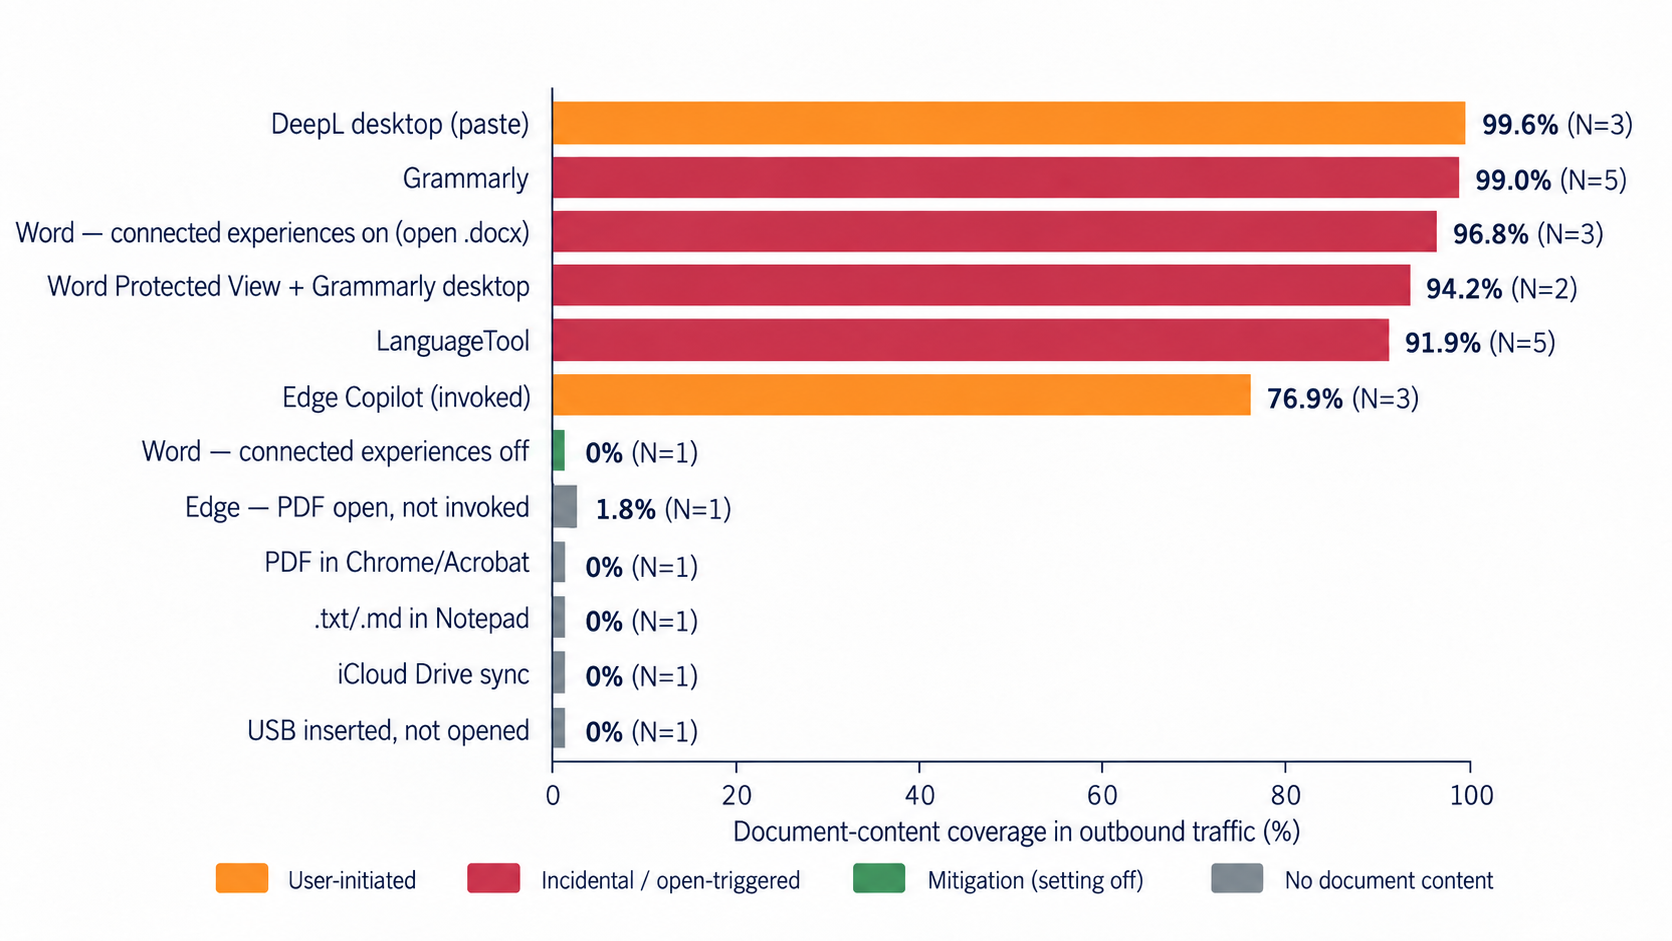
\includegraphics[width=\columnwidth]{figures/fig_spectrum.png}
  \caption{Document-content coverage in outbound traffic, by user action and surface.
  Exact run counts $N$ are shown per bar; single-run rows are individual observations, not
  repeatability estimates. Edge/Copilot is a lower bound (some channels were
  certificate-pinned). The ``no document content'' class means no attributable
  document-specific content: the passive Edge bar's 1.8\% is a generic boilerplate phrase,
  not a planted secret.}
  \Description{Bar chart of document coverage per condition ordered by user action, from passive storage at zero percent through incidental exposure in Word and browser extensions above ninety percent to user-initiated DeepL and Copilot use; run counts are printed on each bar.}
\label{fig:action-spectrum}
\end{figure}

\subsection{Permissions and the exposure channel}
\label{sec:permissions}

A natural question is whether these tools reach beyond text into device sensors. Auditing
the Windows capability store (mic, camera, location, contacts, full-disk access, and the
rest) and each extension's declared permissions showed that none of the writing or
translation tools (Grammarly, LanguageTool, DeepL) holds microphone, camera, or
broad-filesystem access: the microphone and camera belong only to communication, voice,
and meeting apps. What the writing tools do hold is the browser's ``Access your data for all
websites'' host permission, which is precisely the capability
that lets a content script read every editable field~\citep{mozilla2024permissions}. The
exposure channel is therefore the text a user types or pastes, granted through this
all-sites content permission, not audio or video surveillance. In our setup the always-on
clients (Grammarly for Windows, DeepL desktop) launched at start-up, so they are already
running before the user does anything.

\section{Discussion}
\label{sec:discussion}

The clearest single result is the canary rather than the percentage. A unique
token that existed only inside a document marked ``\textsc{do not forward}'' was found,
seconds after an ordinary paste, in traffic bound for two companies' servers, placed
there by software the user installed once and forgot. Server-side analysis requires the
text to be uploaded, and both vendors
document that they process user text~\citep{grammarly2025privacy,languagetool2025privacy}.
The finding is the gap between that design and what a user, told ``don't share this with
AI,'' would expect when they paste a paragraph into an unrelated field, a gap best
understood as a breach of contextual integrity~\citep{nissenbaum2004contextual}.

This distance matters because the exposure is (a) invisible: there is no prompt, no
click, no confirmation; (b) complete: essentially the whole document, not a
fragment; and (c) highly repeatable within the tested setup: it happened on every run. For
an individual handling regulated data (health, legal, financial) the implication is direct:
the writing assistants we tested are incompatible with a ``do not share''
instruction unless explicitly disabled, and disabling them is not the default. It also
matters when a tool sends: the user-initiated and the incidental transfers
distinguished in Section~\ref{sec:modes} carry different risk, and the grammar
checkers we tested are the silent, background kind that transmit the moment text appears.
Table~\ref{tab:rq} summarises this across surfaces: exposure differs little in extent once
content enters a watched surface, but the trigger, the required user action, and the
available off-switch differ markedly.

\subsection{Documented versus measured behaviour}
\label{sec:disclosure}
Because the tools behave as designed, it is fair to ask what the finding adds to the
vendors' own documentation. Table~\ref{tab:disclosure} sets, for each content-bearing
channel, what the vendor documents against what we measured. Three differences recur.
First, granularity: the documentation describes \emph{that} text is processed to provide
the service, whereas the measurement shows the \emph{whole field} is transmitted at the
moment of paste, before any suggestion is shown or accepted, and for Word before any edit is
made. Second, scope: the documentation is written for a user of the product, whereas the
transmission also captures text the user entered for an unrelated purpose in a field the
product happens to watch. Third, linkability: Grammarly's transmission carries an account
token alongside the text (Section~\ref{sec:linkability}), which the user-facing description
of the feature does not make apparent. None of this contradicts the documentation; the gap
is between what a document says and what a user told ``do not share'' would infer from it.
\begin{table}
\caption{Documented versus measured behaviour per channel. The ``Documented'' column
paraphrases each vendor's cited privacy documentation (access dates in the references); the
``Measured'' column reports this study's findings.}
\label{tab:disclosure}
\small
\begin{tabular}{@{}>{\raggedright\arraybackslash}p{1.9cm}>{\raggedright\arraybackslash}p{2.7cm}>{\raggedright\arraybackslash}p{3.3cm}@{}}
\toprule
\textbf{Channel} & \textbf{Documented} & \textbf{Measured} \\
\midrule
Grammarly ext. & processes the user's text on its servers to provide writing suggestions~\cite{grammarly2025privacy} & whole field (99.0\%) on paste, before any suggestion; account token attached \\
LanguageTool ext. & by default sends text to its servers to be checked and states it is not stored~\cite{languagetool2025privacy} & whole field (91.9\%) on paste, before any suggestion; no account identifier \\
Word connected exp. & experiences that analyse content process it in the cloud and can be turned off in Account Privacy settings~\cite{microsoft2026connectedexp} & 96.8\% on open, no edit or submission; 0\% with the setting off \\
Grammarly desktop & offers suggestions in supported desktop applications~\cite{grammarly2025privacy} & 94.2\% from a Protected View window, no user action \\
Edge Copilot & processes page content the user provides when Copilot is invoked~\cite{microsoft2026copilotprivacy} & $\geq$76.9\% and all secrets, before the model's reply declined to reveal them \\
\bottomrule
\end{tabular}
\end{table}

\subsection{Regulatory context (EU GDPR)}
Our tests use only synthetic data, so no real personal data is involved; but the same
mechanism matters wherever those fields would hold real personal data. A silent
whole-document upload raises questions under three expectations of the EU's data-protection
law (GDPR, Regulation~(EU)~2016/679): being transparent about where data goes, sending only
the data that is needed, and informing the person the data is about of the third parties
that receive it (Arts.~5, 13, and 14). If the
receiving servers are outside the EU, the law's cross-border-transfer rules (Chapter~V) also
apply. The risk is largest at work, where an employee may paste client data into a consumer
tool that has no data-processing agreement in place (Art.~28). We make no legal ruling ---
whether any specific use is lawful depends on the details --- but the engineering point is
simple: the problem is not only that the data leaves, but that it leaves invisibly, with
nothing telling the user it happened.

\subsection{After transmission}
Our experiment measures transmission, not what
happens afterwards. Once document content leaves the machine it enters the downstream
ecosystem of retention, provider-side processing, model training, and attribute inference
reviewed in Section~\ref{sec:related}, expanding the set of systems that can process,
retain, and act on it. These downstream practices vary by provider and configuration and lie
outside our measurement scope; quantifying the network exposure precisely, rather than
trusting vendor assurances, is the necessary first step to reasoning about them.

\section{Limitations}
\label{sec:limitations}

We measured across several surfaces (browser extensions on an isolated Linux VM; desktop,
Office, and operating-system tools on Windows~11, since several desktop tools are unavailable
on Linux), which broadens the range of surfaces examined. Two limits apply. First, traffic
protected by certificate pinning cannot be read (for example
\texttt{*.events.data.microsoft.com} and some Adobe and Google endpoints); content we cannot
decrypt is not counted, so figures from conditions with pinned channels (Edge/Copilot) are
lower bounds, whereas the browser-phase conditions had zero un-interceptable handshakes and
are complete. Interception can itself weaken the observed
connection~\citep{durumeric2017https}; the proxy CA was trusted only in the browser test
profile and, for the host phase, added to the Windows certificate store for the capture
window only, with the raw traffic reported unmodified.

Second, a native application can
use sockets that ignore the system proxy: the Grammarly Windows client on Notepad sent only
telemetry through the proxy while opening a direct connection we could not inspect, so that
case is reported as unmeasured rather than zero; results captured through the proxy (browser
extensions, Office, and Grammarly in Word) are unaffected.

Third, the study is deliberately deep rather than broad. The controlled comparison covers
two extensions in one browser (Firefox ESR) with one document of about 2{,}000 characters;
we have not tested Chromium-based browsers, longer documents that a tool might chunk or
truncate, or the other writing assistants on the market. The host phase used consumer
accounts and a personal Microsoft~365 licence; enterprise tenants, to which Microsoft's EU
Data Boundary and processor commitments apply, and institutional Grammarly licences may
behave differently and were not measured. The connected-experiences-off mitigation and the
passive controls are single-run observations and the Protected View result rests on two
identical runs; they are reported as such and not as repeatability estimates.

Fourth, we observed but did not establish the mechanism by which the Grammarly desktop
client obtained the text of a Protected View window. The client's documented operation on
supported applications is consistent with text access through the operating system's
accessibility interface, which Protected View does not restrict, but we did not verify this
and leave it to future work.

\section{Conclusion and Future Work}
\label{sec:conclusion}

We measured how much of a confidential document leaves the machine when common
LLM-integrated productivity tools are used at their defaults. In the primary browser
experiment, both writing-assistant extensions transmitted all twelve planted identifiers
and nearly all measurable document content, while the identical no-extension baseline
transmitted none. The secondary host probes show that comparable exposure can occur through
other productivity surfaces, but the triggering interaction varies: some transfers follow
explicit user invocation (the DeepL paste, the Copilot summary), others occur when content
enters a background or editor-integrated service (the browser assistants, Word's connected
experiences), and the negative controls show that storage location alone does not cause
exposure. As an answer to the research question, exposure differs little in extent once
content reaches a watched surface---near-total, with all twelve secrets---and differs mainly
in what triggers it and whether the user can switch it off. The tools behave as designed; the
finding is how far that design sits from the
expectation of a user told not to share the file. The unifying result is that exposure is
surface-dependent: content leaves the machine when it enters a surface an LLM-integrated
service watches, not because of where the file is stored. This moves the user's real point
of control to before the text enters such a surface. That turning off one Office setting
removed the largest incidental transfer, a single-run observation, indicates the behaviour
is a configuration choice, not a technical necessity.

\textbf{Future work.} The immediate extensions follow from the limitations above: widening
the controlled comparison to further assistants and to Chromium-based browsers, replacing
the bare local page with a real submission form, adding PDF viewers with built-in
assistants, measuring an enterprise tenant, and bringing the single-run conditions to three
runs. A further step is to classify the transmitted data by type: an
automatic labelling of which categories of personal information (names, contact details,
financial data, identifiers) each tool transmits. This would extend the automated PII sweep
with Microsoft Presidio~\citep{microsoft2018presidio}, already used here to surface account
identifiers travelling alongside the document, into a full per-category inventory across the
captures. A further mechanistic extension remains: dynamic
instrumentation (for example Frida) to read certificate-pinned channels that are currently
only a lower bound.

% End of main body (12-page limit). The sections below do not count.

\appendix

\begin{acks}
To be added for the camera-ready version.
\end{acks}

\begin{ethics}
All planted test data is synthetic: no real person, organisation, or system is referenced.
The study measures default-configuration behaviour of legitimately installed software on the
authors' own machine and does not attack the software vendors' systems or other users. Because
the host phase intercepted system-wide traffic, incidental background flows from the
authors' own accounts were also decrypted; only flows relevant to the synthetic-document
experiment were retained for analysis and unrelated incidental background flows were
excluded, the proxy CA was added to the Windows certificate store only for the capture
window and removed afterwards, and the published capture summaries were scrubbed of
incidental account identifiers before release. No responsible-disclosure step was required:
the behaviour we measure is documented by the software vendors and is not a vulnerability.
The study was not submitted to an external ethics panel: it involved no human participants and no real personal data, and measured only software installed on the authors' own devices under the authors' own accounts.
\end{ethics}

\begin{openscience}
The capture and analysis code, the synthetic memo, and the planted-secret list are available
at an anonymised repository\footnote{\url{https://anonymous.4open.science/r/XXXX} (de-anonymised link provided upon acceptance).}.
The raw decrypted captures are not released because the host phase incidentally decrypted background traffic from the authors' own accounts; the scrubbed per-flow scoring summaries that support every figure and table are included.
\end{openscience}

\begin{ai}
The authors used generative AI-based tools to revise the text, improve flow, correct typographical and grammatical errors, and check \LaTeX{} formatting. AI-based tools were not used to design the experiments, collect or analyse the data, or draw conclusions. We have manually verified and are responsible for the accuracy, originality, and integrity of the output of all AI-based tools.
\end{ai}

\bibliographystyle{ACM-Reference-Format}
\bibliography{refs}

\end{document}
